\section{Gangbild anpassungen}
\subsection{Versuch 10}
Training vereinfachter Mixamo Charakter. Lernt zu galoppieren.

\begin{figure}[H]
  \centering
  \begin{tabular}{cccc}
    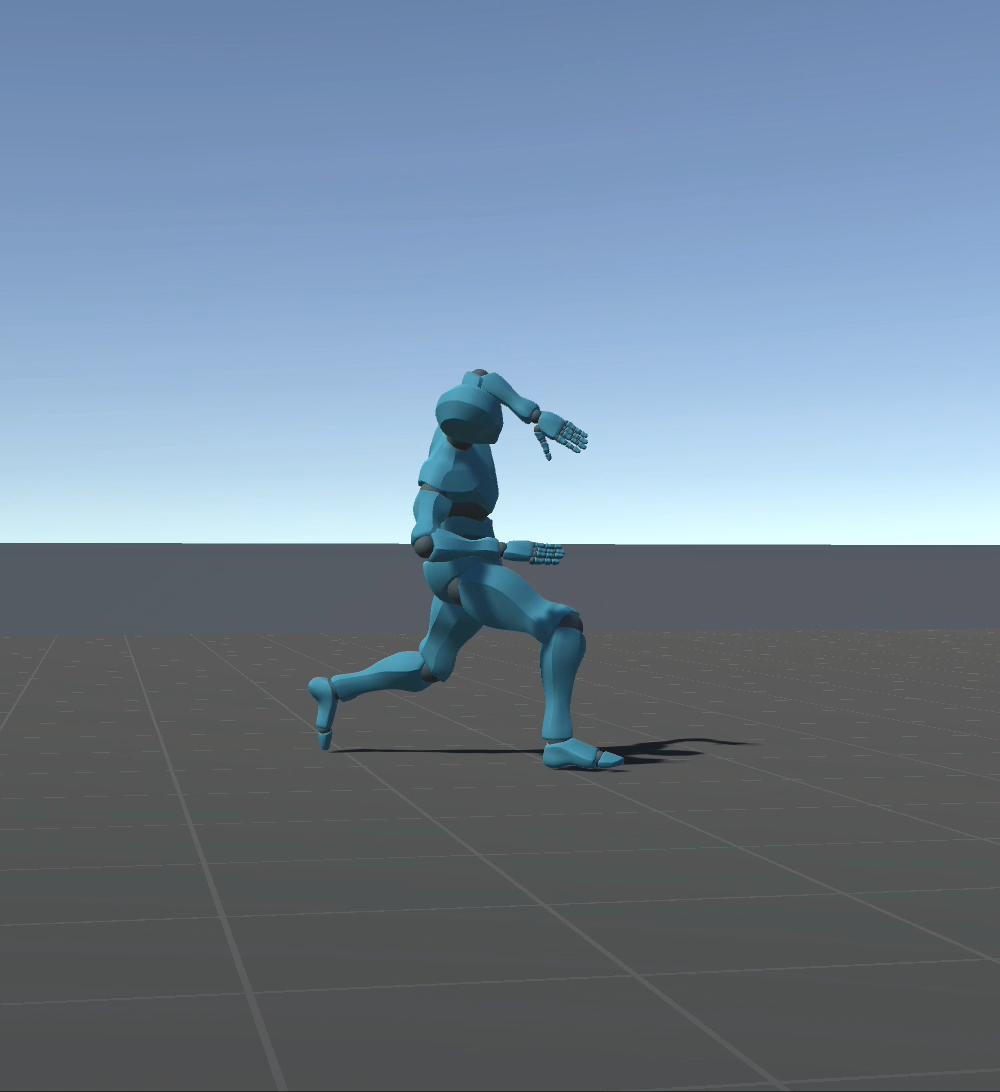
\includegraphics[width=0.2\textwidth]{img/charakter_mixamo_galoppieren1} & 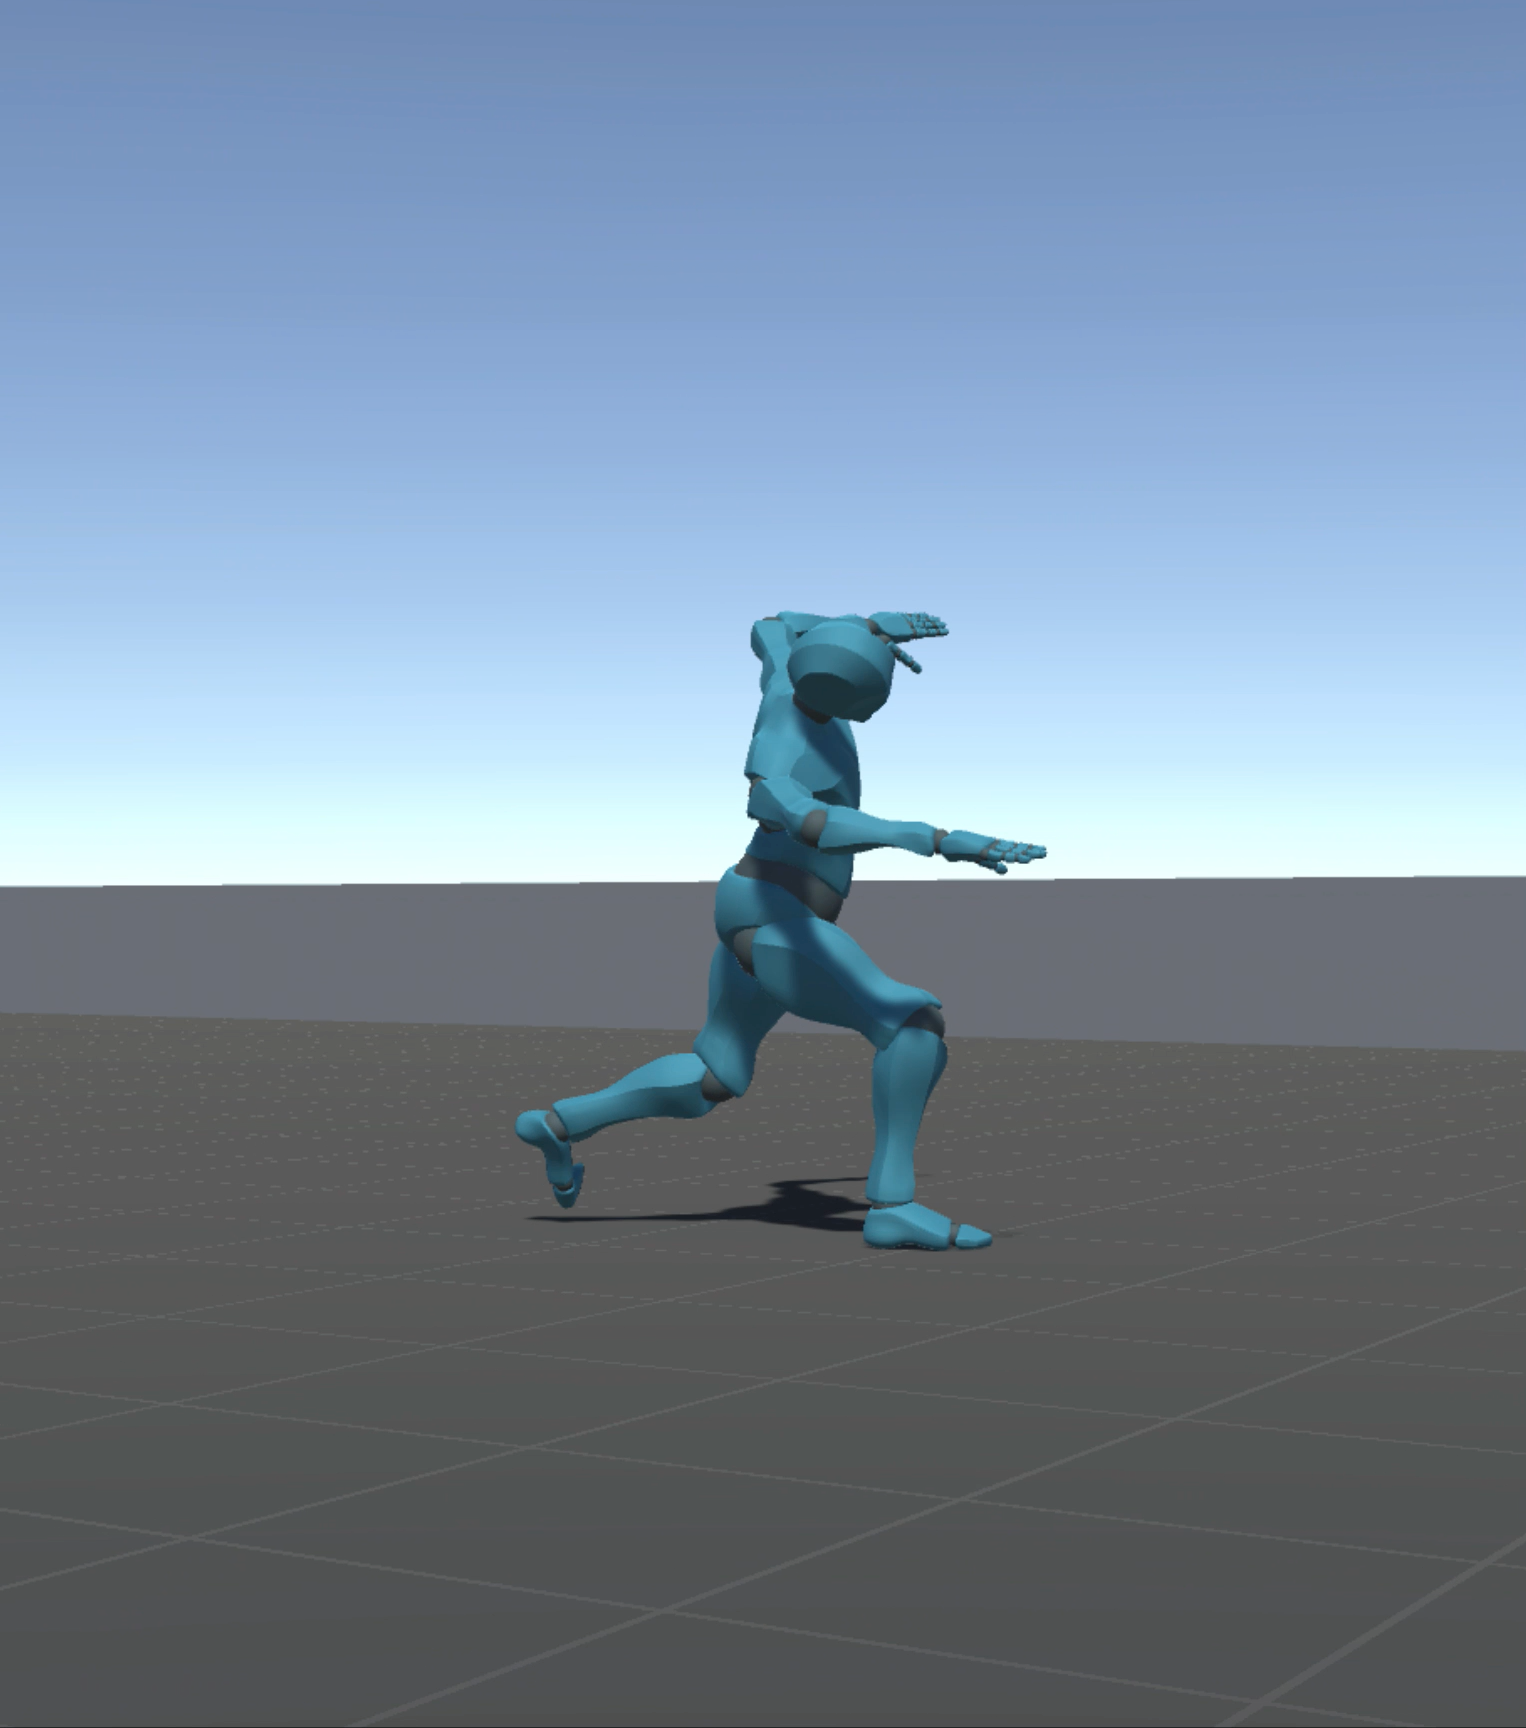
\includegraphics[width=0.2\textwidth]{img/charakter_mixamo_galoppieren2} & 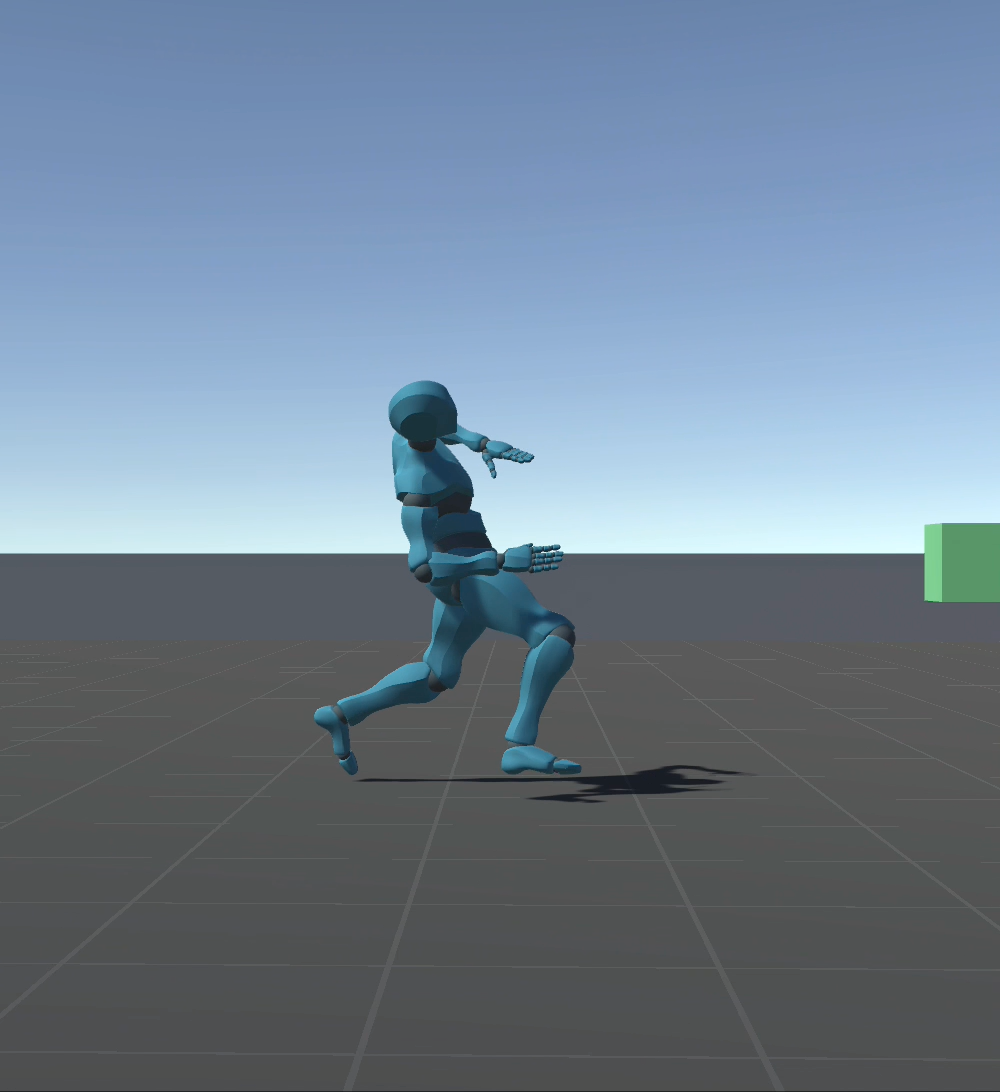
\includegraphics[width=0.2\textwidth]{img/charakter_mixamo_galoppieren3} & 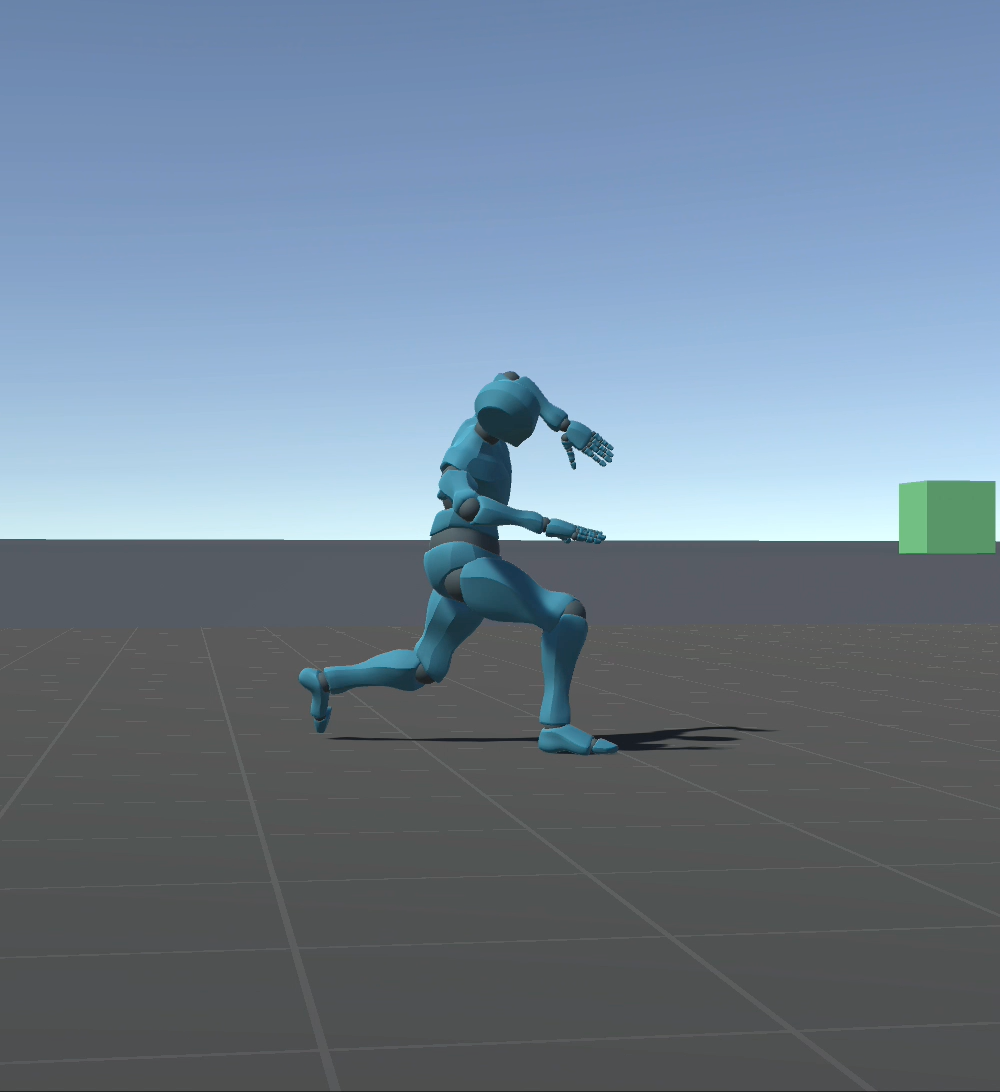
\includegraphics[width=0.2\textwidth]{img/charakter_mixamo_galoppieren4} \\
  \end{tabular}
  \caption{Mixamo Versuch 10 Gangbild}
  \label{fig:mixamo_versuch10_gangbild}
\end{figure}

\subsection{Versuch 11}
Hinzufügen von Beinwechsel Belohnung. Lernt mit periodischem Beinwechsel zu laufen.

\begin{figure}[H]
  \centering
  \begin{tabular}{ccc}
    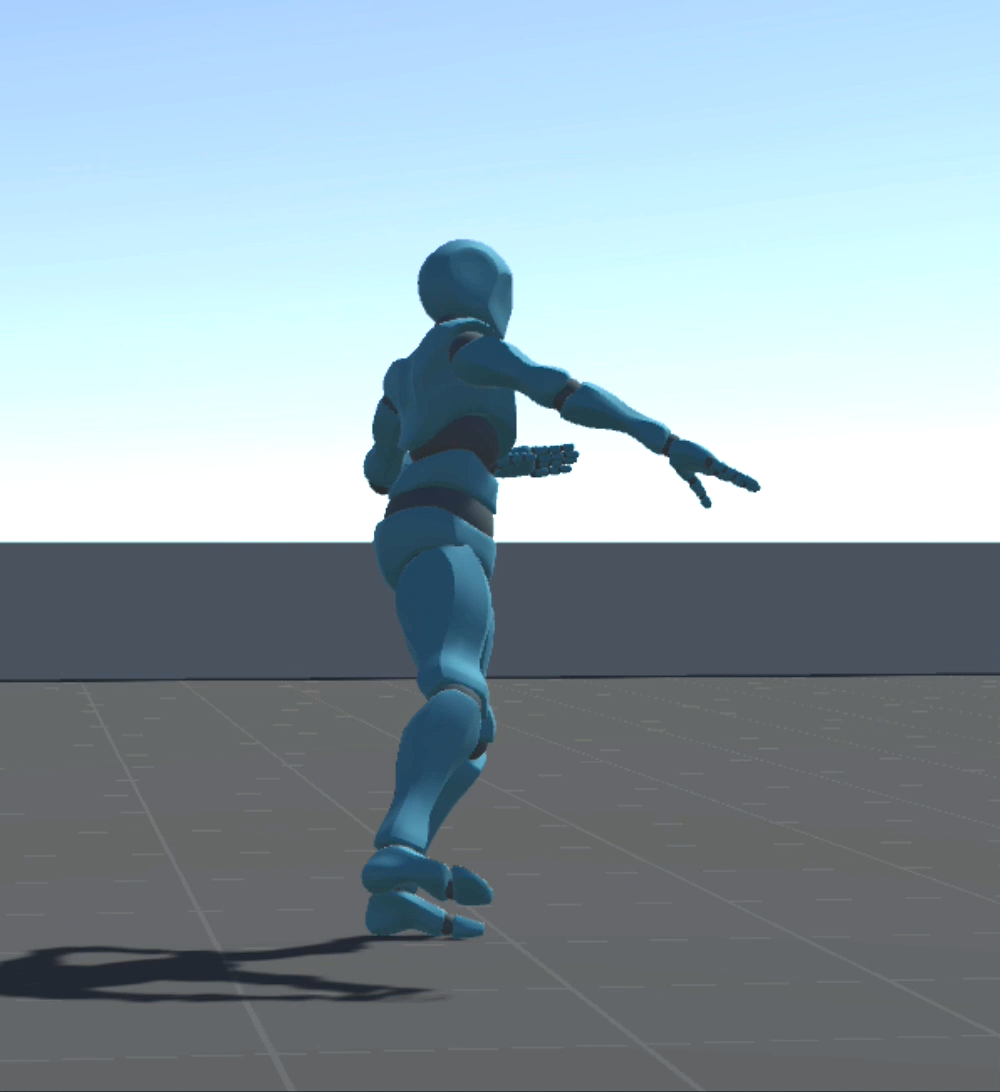
\includegraphics[width=0.27\textwidth]{img/charakter_mixamo_laufen1} & 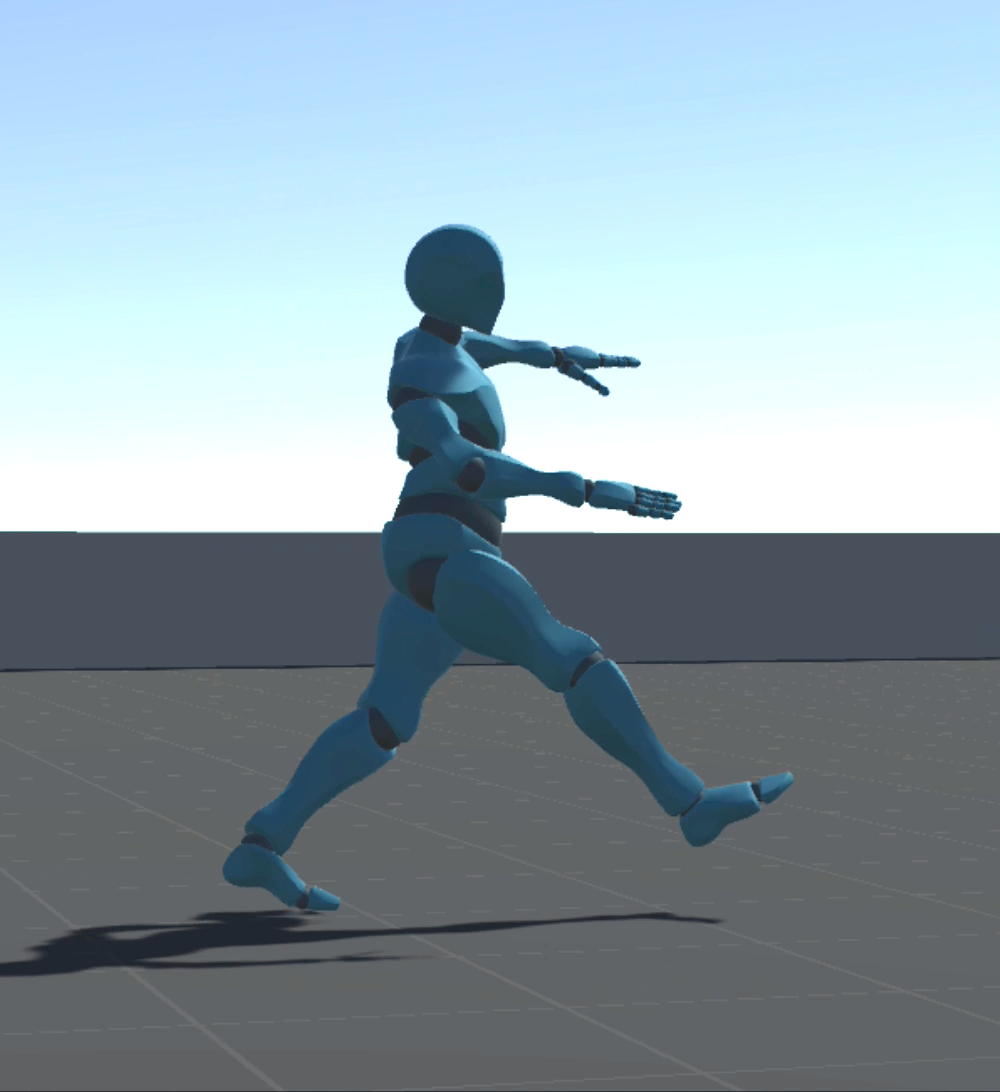
\includegraphics[width=0.27\textwidth]{img/charakter_mixamo_laufen2}  & 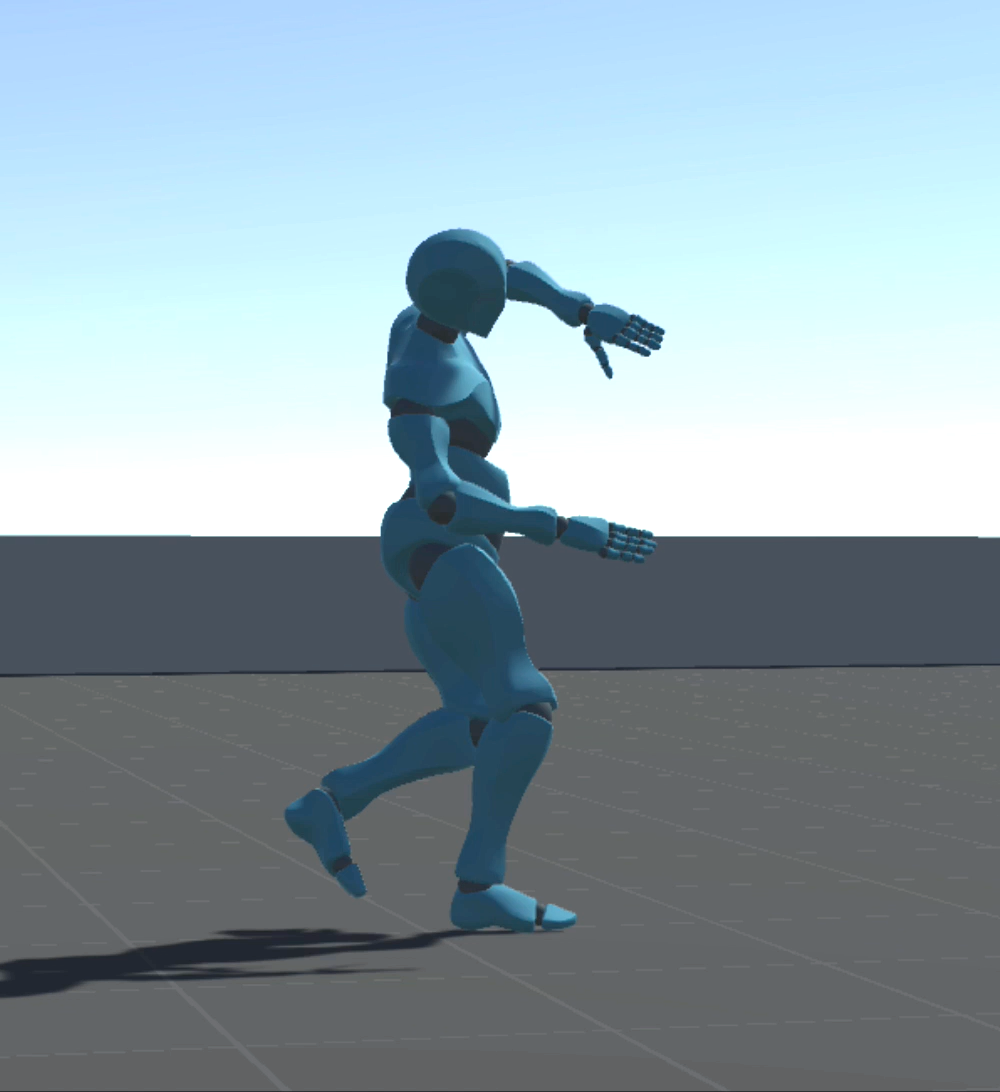
\includegraphics[width=0.27\textwidth]{img/charakter_mixamo_laufen3} \\
    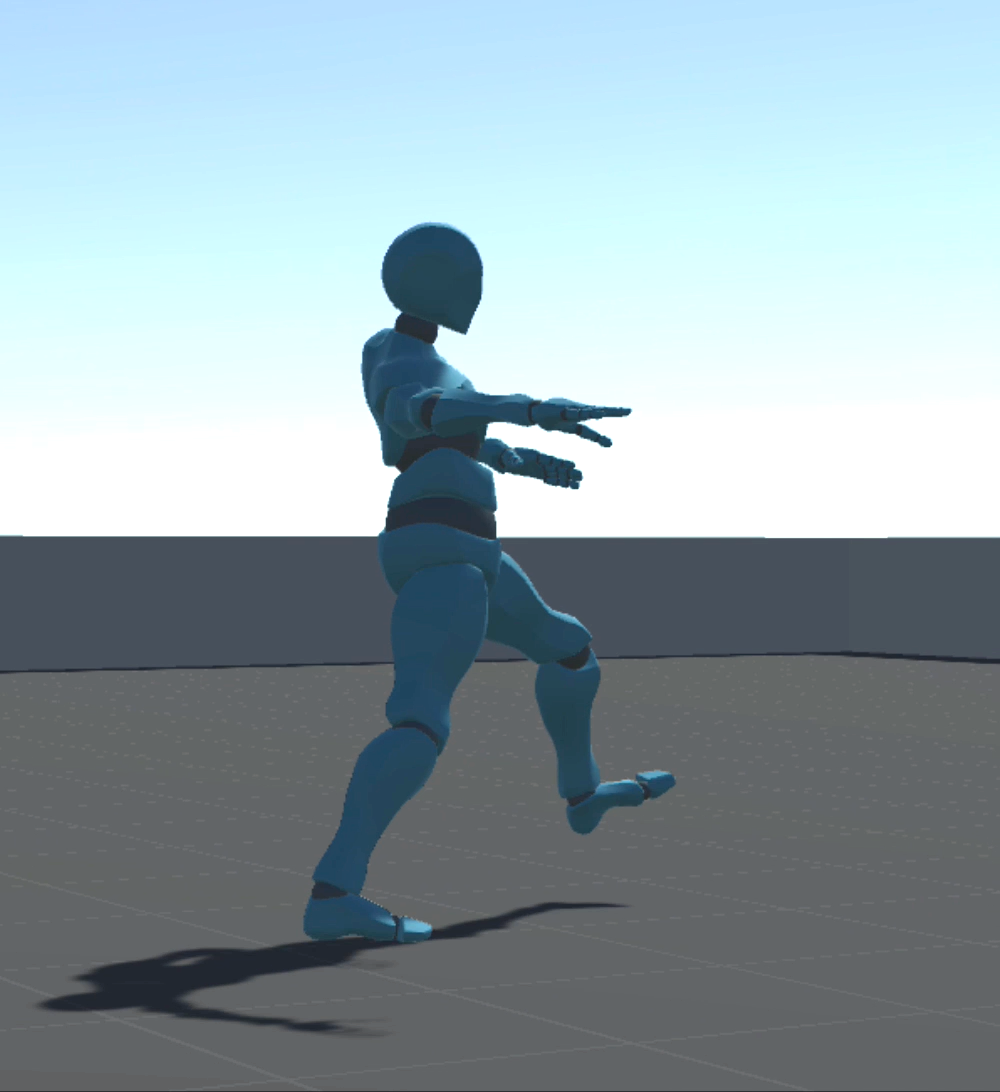
\includegraphics[width=0.27\textwidth]{img/charakter_mixamo_laufen4}  & 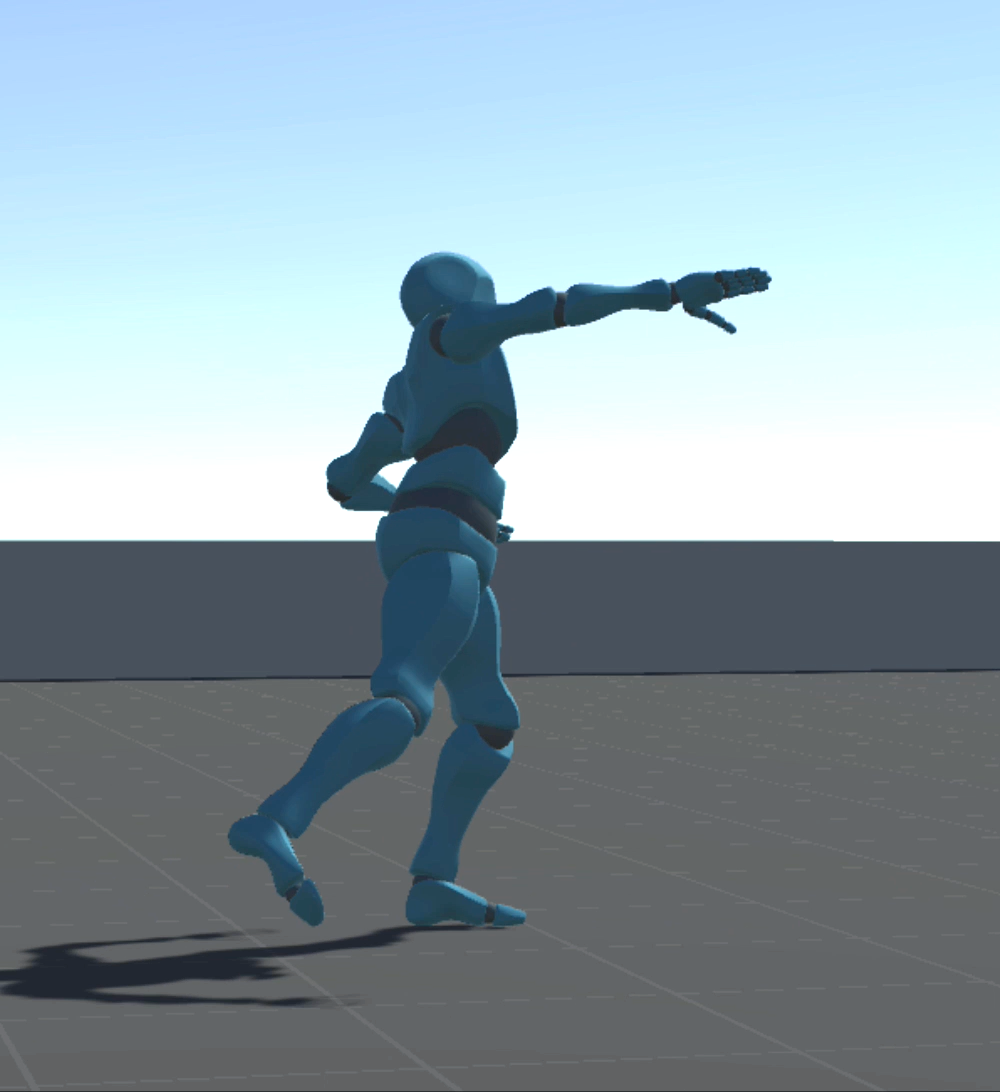
\includegraphics[width=0.27\textwidth]{img/charakter_mixamo_laufen5}  & 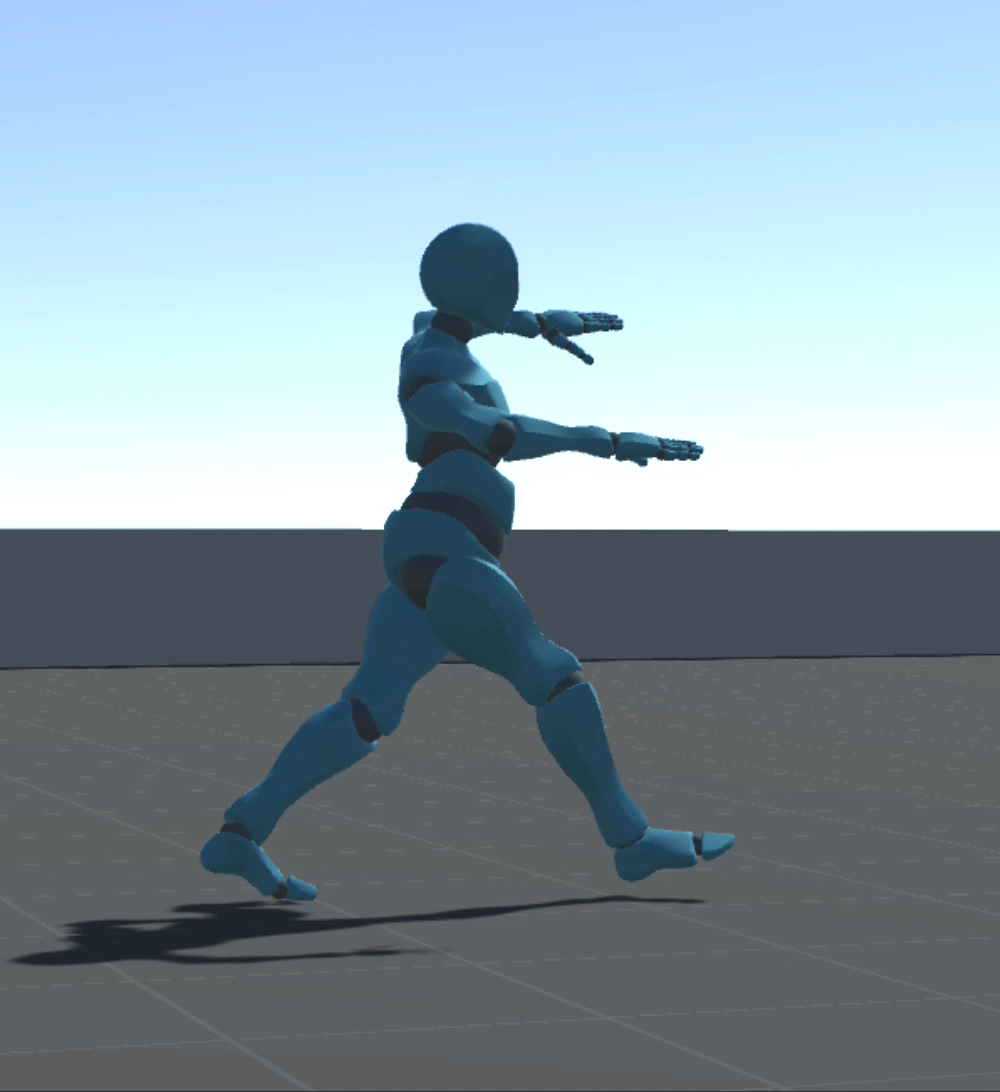
\includegraphics[width=0.27\textwidth]{img/charakter_mixamo_laufen6} \\
  \end{tabular}
  \caption{Mixamo Versuch 11 Gangbild}
  \label{fig:mixamo_versuch11_gangbild}
\end{figure}

\subsection{Versuch 12}
Energiespar Belohnung um Gangbild natürlicher zu machen. Gangbild wird natürlicher aber Arme sind noch sehr starr und nah am Körper.

\begin{figure}[H]
  \centering
  \begin{tabular}{ccc}
    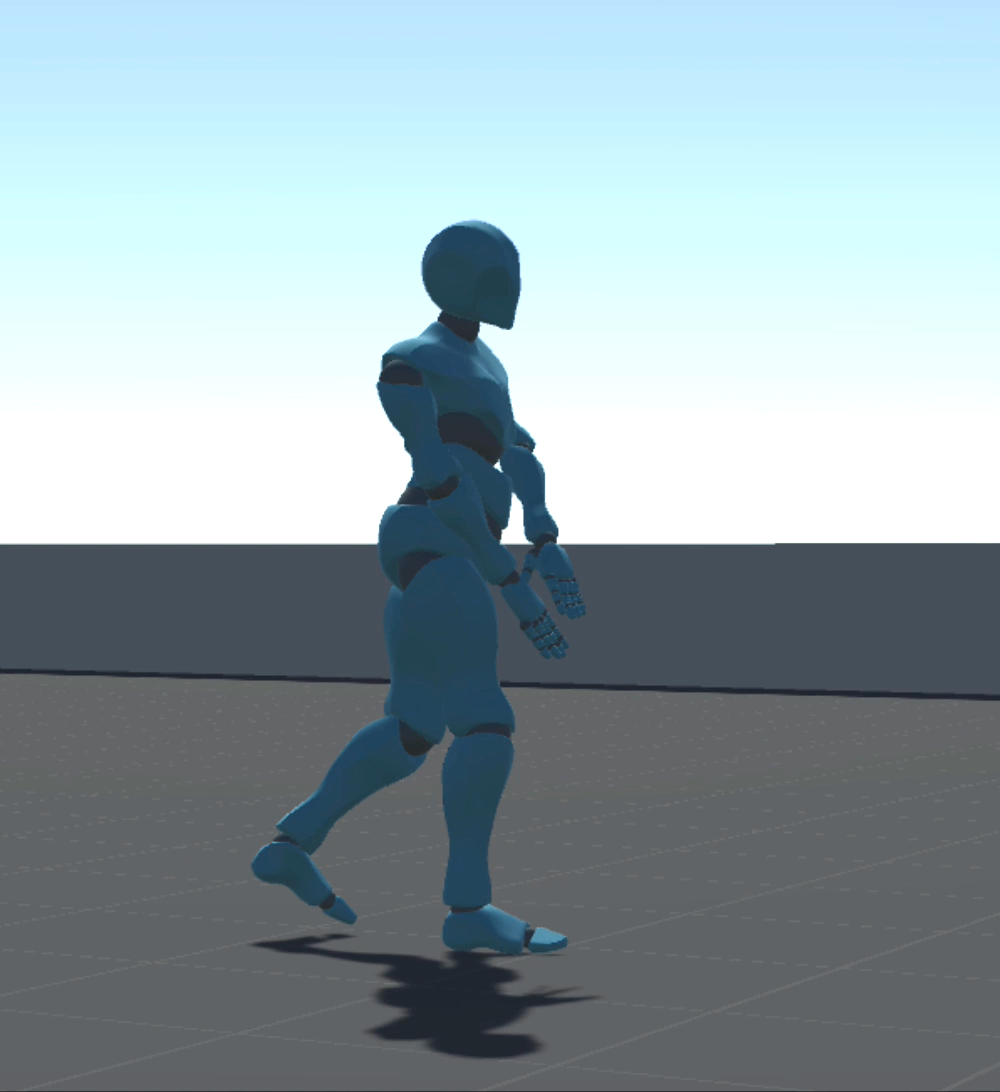
\includegraphics[width=0.27\textwidth]{img/charakter_mixamo_laufen_energiespar1} & 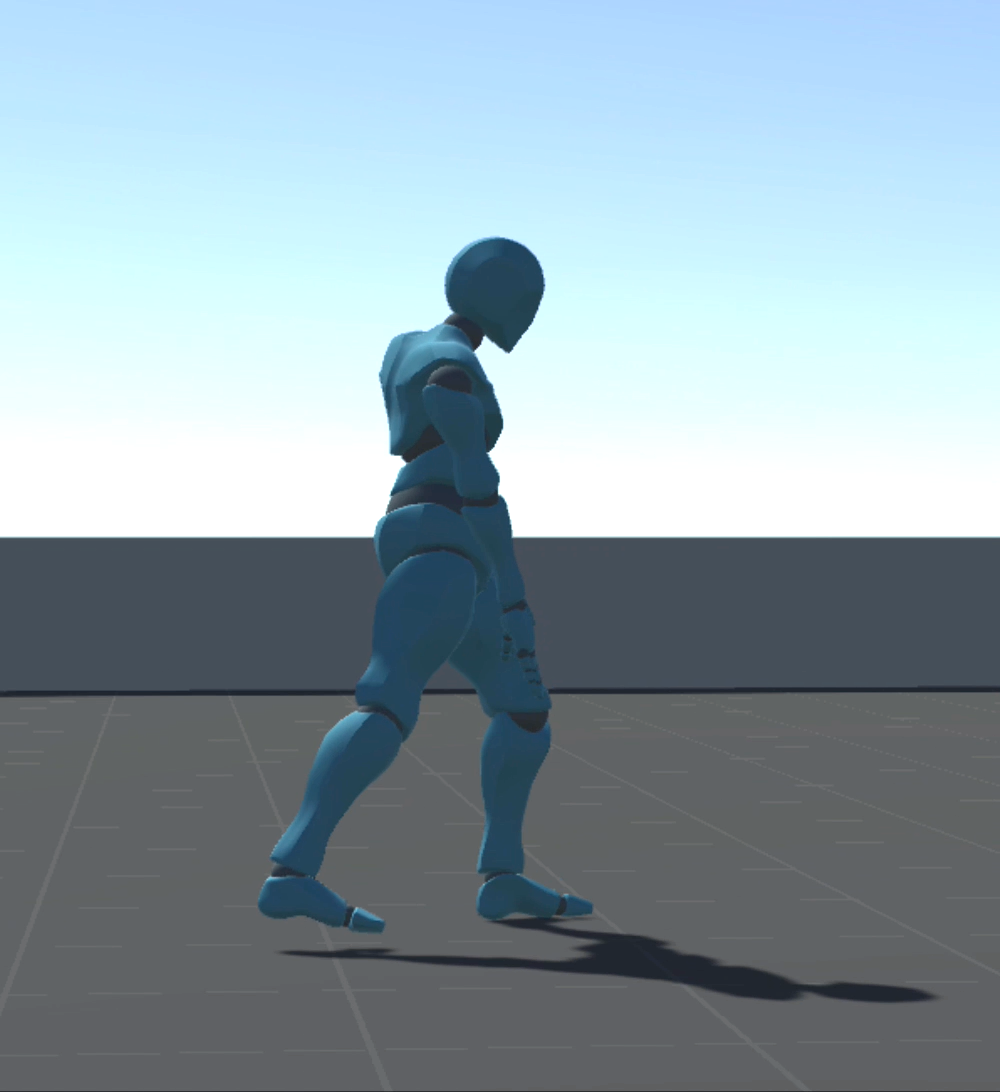
\includegraphics[width=0.27\textwidth]{img/charakter_mixamo_laufen_energiespar2}  & 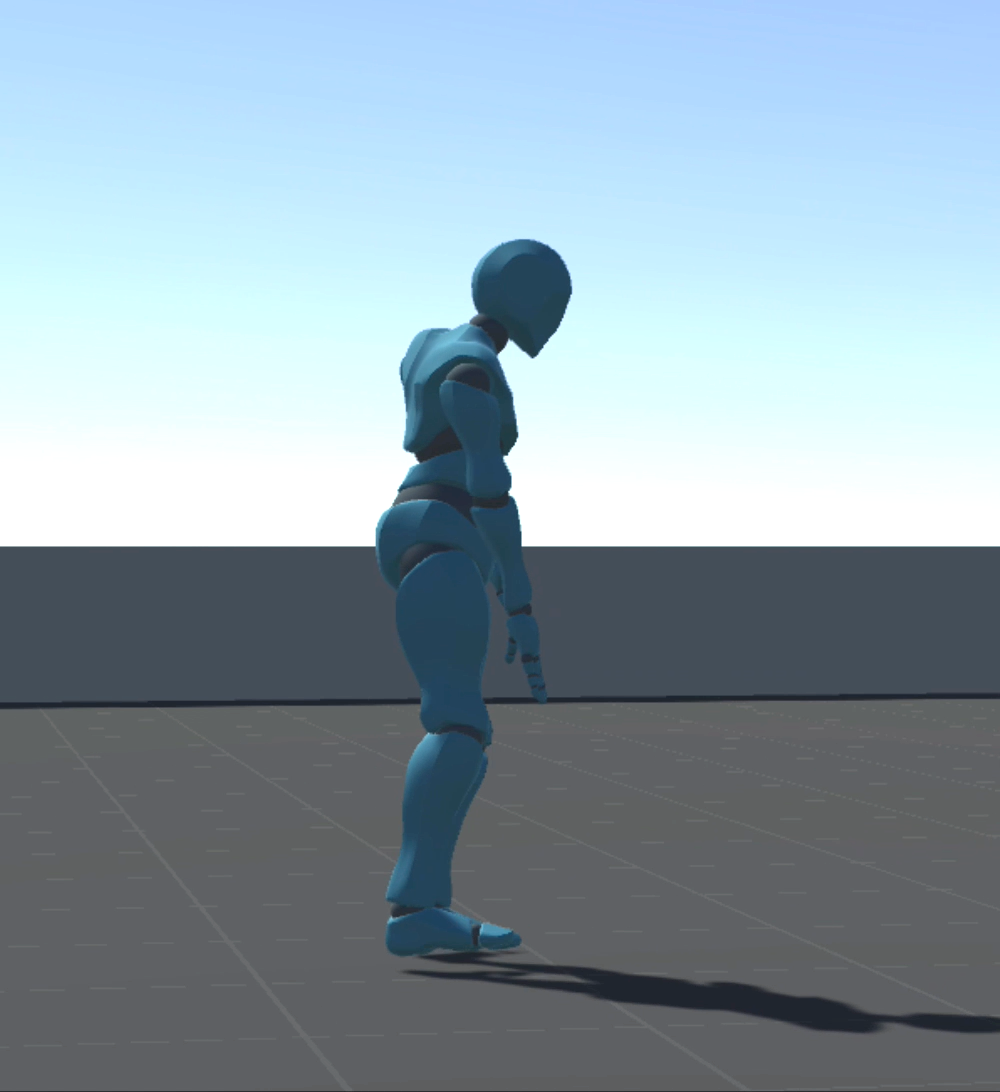
\includegraphics[width=0.27\textwidth]{img/charakter_mixamo_laufen_energiespar3} \\
    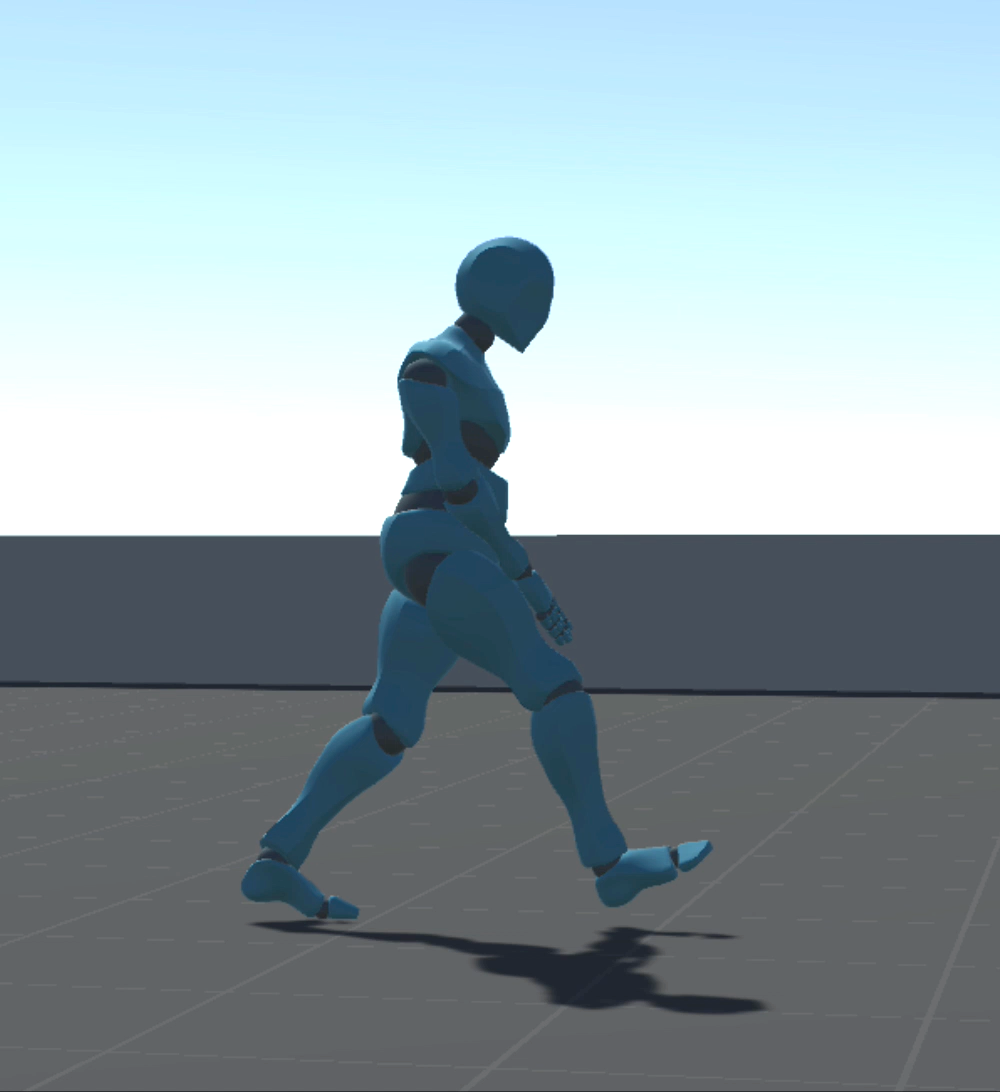
\includegraphics[width=0.27\textwidth]{img/charakter_mixamo_laufen_energiespar4}  & 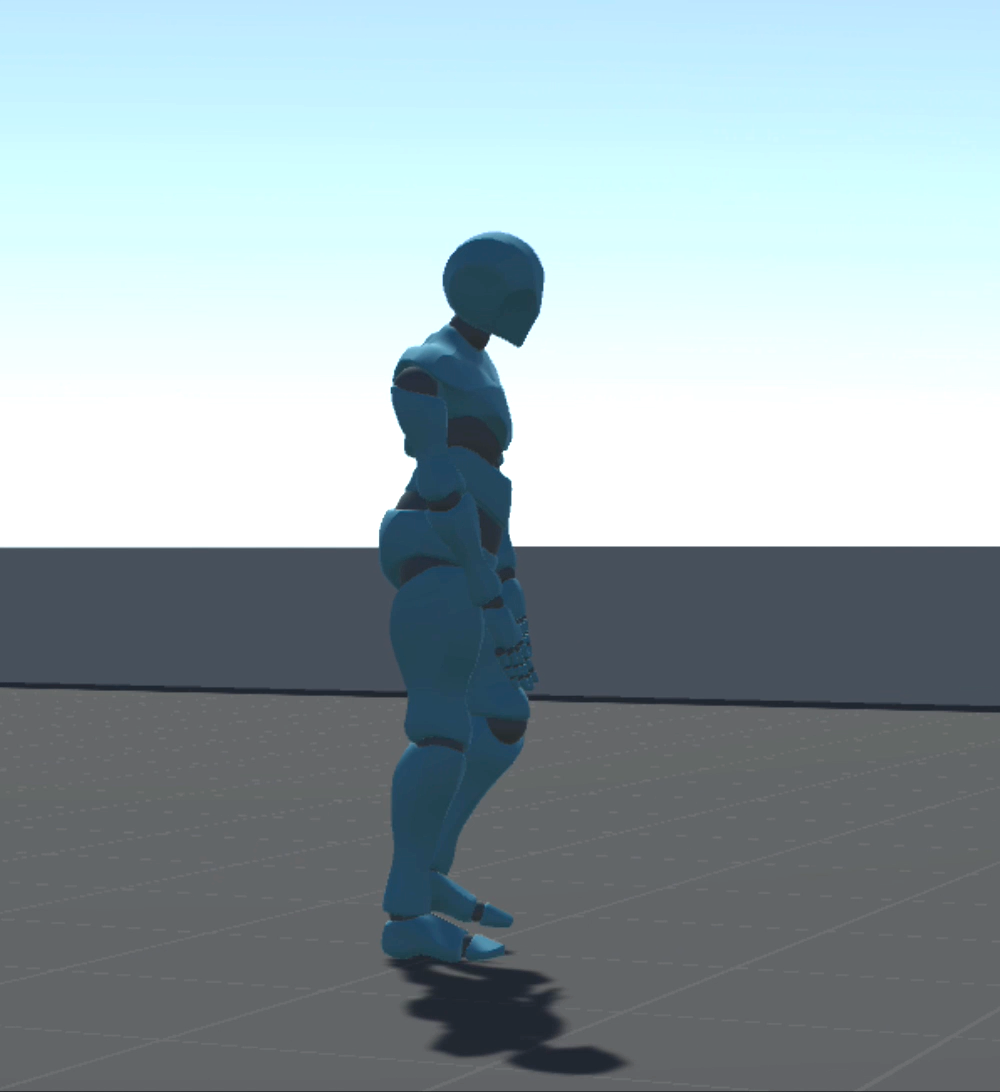
\includegraphics[width=0.27\textwidth]{img/charakter_mixamo_laufen_energiespar5}  & 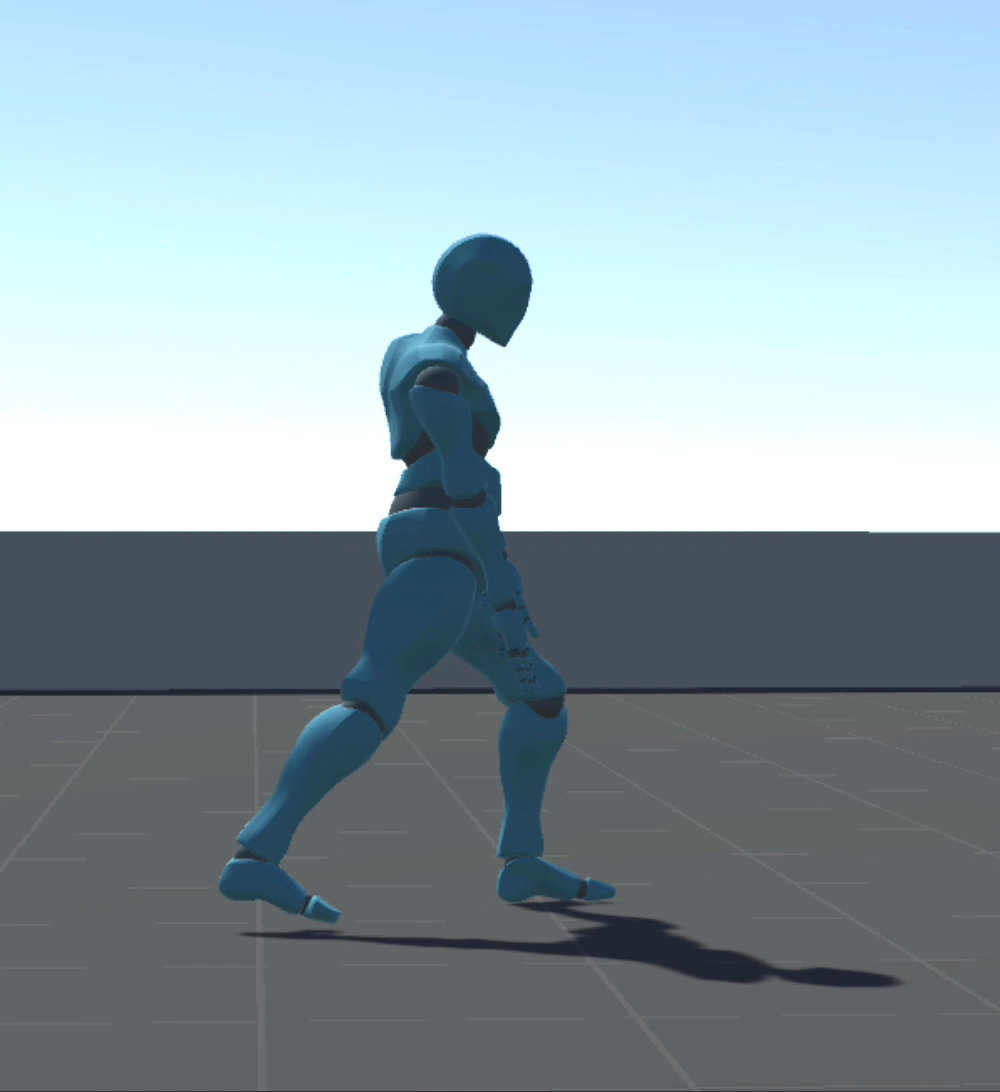
\includegraphics[width=0.27\textwidth]{img/charakter_mixamo_laufen_energiespar6} \\
  \end{tabular}
  \caption{Mixamo Versuch 12 Gangbild}
  \label{fig:mixamo_versuch12_gangbild}
\end{figure}

-Beinwechsel Belohnung um galoppieren zu vermeiden -> funktioniert
-Leistungsminimierung Belohnung um laufverhalten natürlicher zu machen -> funktioniert nur arme sind sehr nah und starr am Körper
-